\documentclass[times, twoside]{zHenriquesLab-StyleBioRxiv}

% Please give the surname of the lead author for the running footer
\leadauthor{CellMap Project Team} 

\begin{document}

\title{Subcellular Structures at Scale: ML based segmentations in vEM in whole tissues}
\shorttitle{CellMap vEM Workflow}

% Use letters for affiliations, numbers to show equal authorship (if applicable) and to indicate the corresponding author

\author[1]{David Ackerman}
\author[1]{Misha Ahrens}
\author[1]{Davis Bennett}
\author[1]{Christopher Bleck}
\author[1]{John Bogovic}
\author[1]{Marley Bryant}
\author[1]{Teng-Leong Chew}
\author[1]{Aparna Dev}
\author[1]{Daniel Feliciano}
\author[1]{Jan Funke}
\author[1]{Larissa Heinrich}
\author[1]{Harald F. Hess}
\author[1]{Caleb Hulbert}
\author[1]{Wyatt Korff}
\author[1]{Gudrun Irhke}
\author[1]{Sanna Koskela}
\author[1]{Jennifer Lippincott-Schwartz}
\author[1]{Zhe J. Liu}
\author[1]{Henrique Ludwig}
\author[1]{Caroline Mooney}
\author[1]{Woohyun Park}
\author[1]{Kayvon Pedram}
\author[1]{Alyson Petruncio}
\author[1]{Alannah Post}
\author[1]{Stephan Preibisch}
\author[1]{Jacquelyn Price}
\author[1]{Diana Ramirez}
\author[1]{Jeff Rhoades}
\author[1]{Stephan Saalfeld}
\author[1]{Alyssa Stark}
\author[1]{Alia Suleiman}
\author[1]{Ronald D. Vale}
\author[1]{Rebecca Vorimo}
\author[1]{Aubrey V. Weigel}
\author[1]{Marwan Zouinkhi}
\author[1]{Yurii Zubov}
\author[1,\href{mailto:cellmapadmin@janelia.hhmi.org}{\Letter}]{CellMap Project Team}

\affil[1]{Janelia Research Campus, HHMI, 19700 Helix Drive, Ashburn, 20147, VA, USA}
%\affil[$\dagger$]{These authors contributed equally.}
%\affil[ \href{mailto:weigela@janelia.hhmi.org,funkej@janelia.hhmi.org}{\Letter}]
\affil[ \href{mailto:cellmapadmin@janelia.hhmi.org}{\Letter}]{corresponding authors}

\maketitle

%TC:break Abstract
%the command above serves to have a word count for the abstract
\begin{abstract}
Large-scale, high-resolution imaging of subcellular architecture using volume electron microscopy (vEM) unlocks new opportunities for biological discovery—but realizing this potential requires more than just data acquisition. Scalable infrastructure, robust protocols, and trained personnel are critical to extract consistent insight from these complex datasets and make them useful to the broader community. The CellMap Project Team represents a coordinated effort to scale vEM-based segmentation across six dimensions: dataset scale, biological diversity, organelle classification complexity, team training, analytical depth, and open access. Through modular training programs, systematic quality control, and block-wise processing tools, the project has grown from individual cell volumes to tissue-scale annotation across dozens of organisms and sample types. Annotated datasets are openly shared through OpenOrganelle, providing the community with immediate access to high-resolution volumes and voxel-level segmentations. We describe how workflows and infrastructure evolved to support this scaling effort, with a focus on designing datasets that are tailored for specific biological insight yet structured for broad reuse. By scaling people, protocols, and pipelines in parallel—and committing to open data practices—the CellMap Project Team provides a model for reproducible, high-resolution cellular mapping at scale.
\end{abstract}
%TC:break main
%the command above serves to have a word count for the abstract

\begin{keywords}
volume electron microscopy | deep learning | machine learning | segmentation | big data | open source | team science
\end{keywords}

\begin{corrauthor}

\texttt{\href{mailto:cellmapadmin@janelia.hhmi.org}{cellmapadmin@janelia.hhmi.org}}
\end{corrauthor}

\section*{Introduction}

Volume electron microscopy (vEM) enables the visualization of cellular ultrastructure at nanometer resolution, offering an unprecedented lens into the internal organization of cells. Yet the transition from beautiful imagery to biological understanding is far from trivial. Scalable workflows are essential—not just for acquiring large volumes, but for annotating them meaningfully, analyzing them reproducibly, and sharing them with the community.

The CellMap Project Team builds on the Cell Organelle Segmentation in Electron Microscopy (COSEM) initiative, which demonstrated the feasibility of dense organelle segmentation in individual cells. While COSEM showed what was possible, CellMap set out to make those methods more routine and scalable. As the biological focus shifted from isolated cells to complex tissues and diverse organisms, the project required new infrastructure, workflows, and team structures.

This paper outlines how CellMap has grown along six key dimensions of scale: dataset size and quantity, biological diversity, organelle classification complexity, team training, analytical depth, and open access. Each dimension presents different challenges and tradeoffs—but all are essential for turning raw vEM data into reusable biological insight.

Rather than emphasizing any single dataset, we focus here on the broader strategies that enable this scaling: modular annotation protocols, quality control pipelines, structured training, scalable infrastructure, and public data sharing through OpenOrganelle. In doing so, we aim to provide a roadmap for how high-resolution cellular annotation can be extended to larger biological contexts—across tissues, species, and research goals.

\section*{Dimensions of Scaling in CellMap}
Scaling the CellMap Project has required coordinated growth across multiple, interdependent fronts. While dataset volume and size are often the most visible indicators of scale, we have found that meaningful expansion demands attention to six key dimensions: dataset size and quantity, biological diversity, organelle classification, personnel and training, analytical depth, and open access.

\begin{figure}[htbp]
\centering
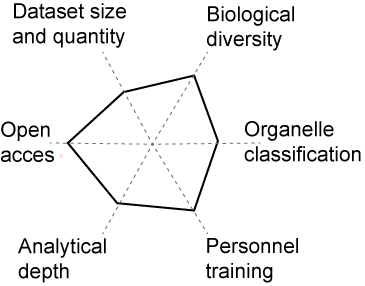
\includegraphics[width=\columnwidth]{Figures/Degrees-of-scaling.png}
\caption{\textbf{Conceptual overview of the six dimensions of scaling in the CellMap Project Team.} This schematic radar plot illustrates the major axes along which the project has scaled: dataset scale, biological diversity, organelle classification complexity, team training, analytical depth, and open access. The plot is qualitative and intended to highlight the multidimensional nature of scaling required for large-scale, high-resolution cellular mapping.}
\label{fig1}
\end{figure}

\subsection{Dataset Size and Quantity}
CellMap has scaled both in the number of datasets and their volumetric size. What began as small, fully segmented single-cell volumes has grown into a collection of dozens of tissue-scale vEM datasets, many of which now exceed tens of teravoxels. This increase in dataset scale reflects advances in sample preparation, imaging, and storage infrastructure, as well as a growing demand for statistically meaningful comparisons across tissues, species, and biological contexts.

The initial proof of concept for whole-cell organelle segmentation came from the COSEM Project Team, which used four tissue culture cell datasets, represented by the pink data points in \ref{fig2}. These early datasets, ranging from 0.122 to 0.257 teravoxels, served as a foundational step in validating the approach.

Currently, 78 publicly available datasets are hosted on OpenOrganelle, spanning a wide range of tissue types and organisms. \ref{fig2} illustrates the distribution of dataset sizes, showing the growth from the initial four COSEM datasets (highlighted in pink) to the full collection (depicted in green). On average, the 55 datasets with segmentations on OpenOrganelle now contain 13.9 ± 40 teravoxels.

To support this expansion, we developed standardized intake pipelines and structured metadata schemas. Scaling at this level also involved adopting blockwise processing and large data visualization tools from the community to improve data handling and visualization.

\begin{figure}[htbp]
\centering
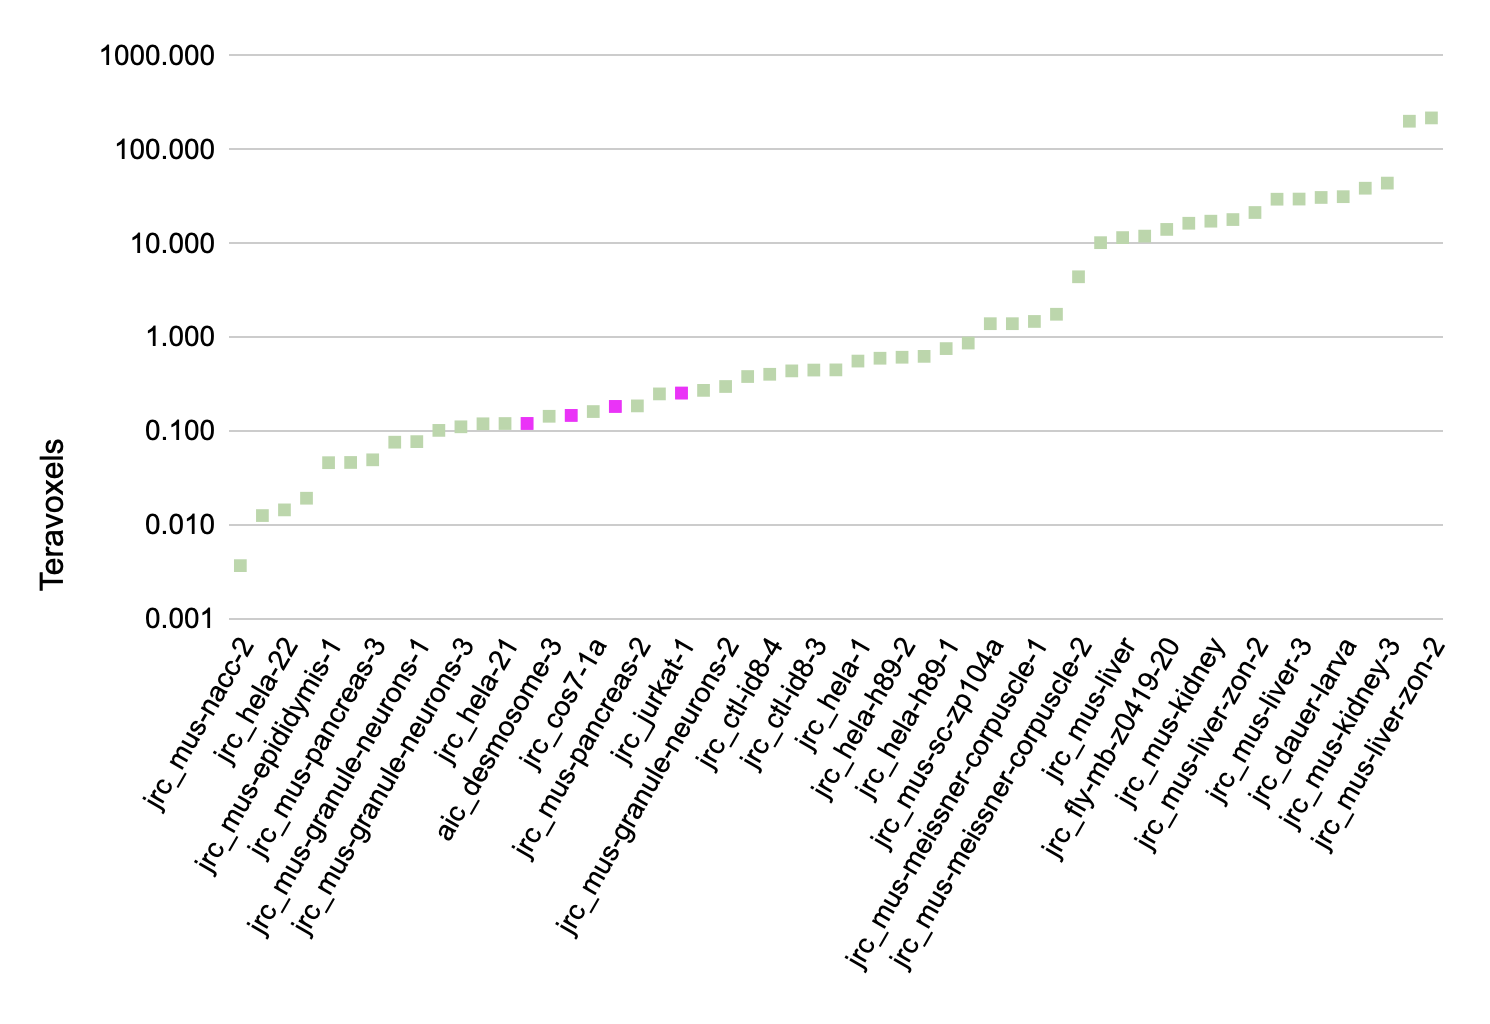
\includegraphics[width=\columnwidth]{Figures/Dataset-size-quantity.png}
\caption{\textbf{Visualization of dataset size and quantity across various CellMap datasets.} This bar plot displays the teravoxel scale of multiple datasets within the CellMap project, showcasing the disparity in dataset sizes and their contribution to the overall imaging effort. The variation in size reflects the project's broad range of biological diversity and tissue types, with a select few datasets representing a significant portion of the total data volume.}
\label{fig2}
\end{figure}

Insert text on data handling pipelines: standardized naming, format conversions, dataset history

Insert text on metadata schema, OME-Zarr, 'soft' metadata

Insert text on current community tools and processes adopted for handling 'big data'

\subsection{Biological and Organismal Diversity}
To generate biologically meaningful insight, CellMap includes data from a wide range of tissues and species, including mouse, fly, zebrafish, and human. This enables generalizable model development and comparative biology but also requires adapting annotation protocols to diverse morphology and membrane contrast characteristics.

\subsection{Organelle Classification Complexity}
The number of labeled organelle classes has grown substantially, now totaling 77 detailed classes including membranes, lumens, and substructures. This supports both fine-grained biological questions and the development of generalizable segmentation models. A strict ontology and visual reference guides ensure consistent application across datasets.

\subsection{Personnel and Training at Scale}
As the CellMap Project expanded, so did the number of annotators involved in segmenting and analyzing vast electron microscopy (vEM) datasets. To support this growth, we developed a modular training curriculum that introduces annotators to organelles in stages of increasing complexity. This structured approach includes milestone-based evaluations and expert reviews, ensuring that annotators can consistently produce high-quality annotations across diverse biological contexts, from isolated cells to complex tissue samples.

\begin{figure}[htbp]
\centering
\includegraphics[width=\columnwidth]{Figures/Training-Workflow.png}
\caption{\textbf{Training Workflow for Annotators.} This figure illustrates the modular training program that annotators go through, beginning with simpler organelles and progressing to more complex structures. The workflow ensures annotators consistently apply the correct protocols and make systematic choices in segmentation.}
\label{fig5}
\end{figure}

The most important part of the training program is that it provides a system for annotators to make consistent choices. While there is inherent ambiguity in vEM data, and misclassification of organelles is inevitable due to the lack of protein specificity and labeling markers, our goal is to ensure that annotators consistently apply the same decisions when faced with ambiguous cases. This consistency is key to producing reliable results and minimizing variability in the annotations.

The training curriculum was designed to ensure that annotators gained a deep understanding of the structures they were annotating. The first stage of training introduces annotators to simple, well-defined organelles such as mitochondria, which helps build foundational segmentation skills. As annotators progress, they tackle more complex organelles like the endoplasmic reticulum (ER) and Golgi, which require more nuanced boundary definitions. Finally, annotators are trained to handle the most challenging structures, including multi-component organelles and tissues with varying membrane contrasts. Each module is paired with practical exercises and feedback sessions to ensure that annotators are applying the correct protocols and accurately segmenting structures.

To ensure high-quality training crops, a screening process was implemented. To manage quality and ensure consistency across a growing number of annotators, we employed a rigorous screening process using a GitHub project to track annotation progress. Annotators submit their segmentations via GitHub, where they are organized into issues and reviewed by team leads. This system facilitates continuous feedback, allowing annotators to receive immediate guidance on their work. Version control ensures that each annotation is reviewed and refined before moving forward, while discrepancy tracking helps identify recurring issues, guiding the revision of training materials and protocols. This system has also streamlined collaboration across team members, ensuring alignment on project goals and annotation standards.

Despite these efforts, human annotators inevitably introduce variability. Variability between annotators remains a significant challenge, as differences in how they interpret organelle boundaries can lead to variations in segmentations. These variations can impact downstream analyses of cellular structures. Several factors contribute to this variability, including individual annotator style, dataset-specific factors such as staining and fixation protocols, and the inherent complexity of organelles. Annotators tend to be more consistent when segmenting larger, more distinct organelles, such as mitochondria, where boundaries are easier to define. However, smaller, more complex structures like the Golgi apparatus and endoplasmic reticulum (ER) often exhibit higher variability.

\begin{figure}[htbp]
\centering
\includegraphics[width=\columnwidth]{Figures/Annotator-Variability-Trends.png}
\caption{\textbf{Trends in Annotator Variability Across Organelle Classes.} This figure illustrates how annotation variability differs across organelle classes. Larger, well-defined organelles such as mitochondria show higher agreement between annotators, while structures with complex morphologies like the Golgi and endoplasmic reticulum exhibit higher variability.}
\label{fig3}
\end{figure}

To quantify and address this variability, we introduced several metrics, including the F1 score and mean false boundary distance (MFBD). The F1 score measures overall agreement between annotators by considering both recall and precision, while MFBD quantifies the average distance between boundaries drawn by different annotators, identifying areas with inconsistent boundary placement. These metrics, integrated into a custom tool available on GitHub, allow annotators and reviewers to compare segmentations and track variability across different organelle classes. This tool helps identify areas where variability is most pronounced, guiding further refinement of training protocols and ensuring greater consistency in future annotations.

\begin{figure}[htbp]
\centering
\includegraphics[width=\columnwidth]{Figures/Annotation-Metrics.png}
\caption{\textbf{F1 Score and MFBD Metrics for Annotation Agreement.} This figure shows the distribution of F1 scores and mean false boundary distance (MFBD) across annotators, highlighting areas of high agreement and areas where variability is more pronounced. The metrics provide insight into segmentation quality and are used to guide annotation improvements.}
\label{fig4}
\end{figure}

Through the integration of these strategies into our workflow, we have minimized variability while maintaining the scalability of the project. This approach has allowed us to generate consistent, high-quality annotations across a growing team and increasingly complex datasets.

\subsection{Analytical Depth and Tailoring to Biology}
Not all annotation needs are the same. CellMap balances detailed, multi-class annotations intended for model training with task-specific efforts tailored to biological questions. This flexibility allows datasets to support both focused and broad reuse.

\subsection{Open Access and Community Reuse}
A core aim of CellMap is to make high-resolution data publicly available. All datasets are shared via OpenOrganelle with standardized formats, class ontologies, and associated metadata. These releases support downstream training, benchmarking, and hypothesis generation across the community. Our infrastructure and workflows were designed to maximize accessibility and encourage reuse beyond their original research context.

\section*{Infrastructure and Coordination}
The scale and complexity of CellMap’s datasets required the development of modular, maintainable infrastructure capable of supporting every phase of the workflow—from raw data acquisition to public data release. This infrastructure evolved in tandem with our growing datasets and team, ensuring that tools, compute, and communication could all scale sustainably.

From a software perspective, we built systems to manage annotation projects, track reviewer feedback, visualize volumetric data, and coordinate distributed training of deep learning models. A key element of this infrastructure is DaCapo, our modular segmentation framework that supports flexible experimentation with architectures, loss functions, and training pipelines at scale. DaCapo enables both centralized and remote model development while keeping data and hyperparameters traceable and reproducible.

Data storage and transfer pipelines were also reengineered to accommodate teravoxel-scale volumes. We implemented cloud-based solutions to facilitate large-volume compute, optimized tiling and chunking strategies to improve data access, and deployed custom viewers to enable efficient navigation of large 3D datasets by annotators and reviewers.

Equally critical was building coordination capacity across a growing team of contributors. The CellMap Project includes data generators, annotators, machine learning researchers, software engineers, and biological collaborators—all working in parallel across multiple datasets. To support this, we established shared documentation, weekly cross-functional meetings, and quality control processes that ensure alignment between annotation goals and analysis pipelines. Together, these coordination strategies allow us to move datasets from raw acquisition to open release within weeks, while maintaining consistency in structure definitions, data formats, and review protocols.

\section*{From COSEM to CellMap: A Scaling Perspective}
The CellMap Project evolved directly from the COSEM initiative, which demonstrated the feasibility of complete manual annotation and deep learning-based segmentation of individual cells imaged at nanometer resolution. COSEM was designed as a proof-of-principle: could we segment entire cells, label key organelles, and train models to reproduce those labels with high fidelity? The answer was yes—but the methods and tools developed during COSEM were optimized for relatively small, highly controlled datasets.

In transitioning to CellMap, we expanded the scope from single-cell volumes to full tissues, from a handful of organelle classes to over 40, and from internal exploratory work to datasets intended for open community use. This shift required more than additional people or compute—it required a strategic rethinking of the entire workflow to ensure that new contributors could be trained efficiently, results could scale without quality loss, and data could be structured in ways that enabled reuse and reproducibility.

Just as importantly, we shifted our framing—from solving a technical segmentation challenge to supporting biological discovery at scale. This meant tailoring our annotation and modeling efforts to the questions at hand: if a collaborator was primarily interested in mitochondrial abundance across liver zones, we could prioritize those structures. But we also recognized that the datasets we were generating contained far more information than any single project required. As a result, we adopted the mindset that every dataset should be annotated as completely and consistently as possible—whether for immediate use or future reanalysis—turning each volume into a reusable community resource.

\section*{Conclusion}
Scaling in biological imaging is often described in terms of data volume or computational throughput—but the CellMap Project illustrates that true scaling requires much more. It involves building resilient workflows, growing and training teams, tailoring analysis to biology, and designing infrastructure that enables consistent and sustainable progress across diverse projects.

We have demonstrated that it is possible to operate at scale without sacrificing quality. We routinely generate, annotate, and analyze datasets comprising tens of teravoxels, across dozens of tissues and organisms, with an expanding organelle ontology and a growing team. Through structured training protocols, robust infrastructure, and clear coordination practices, we’ve created a model for large-scale cellular mapping that serves both individual research questions and the broader scientific community.

These practices have also laid the foundation for broader community-facing efforts. Curated subsets of annotated volumes have been assembled to support segmentation benchmarking and model development, though these efforts are detailed in separate publications. Collectively, these resources reflect a commitment to building datasets that serve both immediate biological inquiry and long-term community use.

Significant challenges remain. Whole-cell segmentation in dense tissue remains difficult, particularly for rare or morphologically variable structures. Integrating multimodal data, supporting fully remote collaboration, and advancing generalization across biological contexts are all areas that require continued investment and innovation.

Nonetheless, CellMap offers a blueprint for scaling—not just in size, but in scope, sustainability, and impact. By investing in people and processes as seriously as we invest in data and compute, we’ve shown that it’s possible to produce high-quality, high-resolution, and high-value datasets that serve both immediate projects and the long-term advancement of cell biology.

\begin{acknowledgements}
We would like to express our gratitude to all the contributors to our GitHub repository. Their valuable input, insightful feedback, and collaborative spirit have significantly enhanced the quality of DaCapo. We appreciate the time and effort invested by each contributor in reviewing code, suggesting improvements, and sharing their expertise. This work would not have been possible without their collective contributions. This work was supported by Howard Hughes Medical Institute, Janelia Research Campus.
\end{acknowledgements}

\begin{contributions}
W.P. and J.F. conceived and initially implemented DaCapo. J.L.R. and M.Z. lead subsequent development and testing, including blockwise processing and documentation, as well as preparing this manuscript. D.G.A., C.M.M., D.A., L.H., D.B., Y.Z., and the rest of the CellMap Project Team contributed to general development and review of the project. A.V.W. and J.F. oversaw general project development. A.V.W., D.G.A., and D.B. gave meaningful contributions to the preparation of this manuscript. The CellMap Project Team during this time was: David Ackerman, Emma Avetissian, Davis Bennett, Marley Bryant, Hannah Nguyen, Grace Park, Alyson Petruncio, Alannah Post, Jacquelyn Price, Diana Ramirez, Jeff Rhoades, Rebecca Vorimo, Aubrey Weigel, Marwan Zouinkhi, Yurii Zubov. Misha Ahrens, Christopher Beck, Teng-Leong Chew, Daniel Feliciano, Jan Funke, Harald Hess, Wyatt Korff, Jennifer Lippincott-Schwartz, Zhe J. Liu, Kayvon Pedram, Stephan Preibisch, Stephan Saalfeld, Ronald Vale, and Aubrey Weigel were part of the CellMap Steering Committee.
\end{contributions}

\begin{code}
The codebase is available on the GitHub repo: \href{https://github.com/janelia-cellmap/dacapo}{github.com/janelia-cellmap/dacapo}
\end{code}

\begin{supplementary}
Installation instructions, tutorials, and extended documentation for DaCapo is available on \href{https://janelia-cellmap.github.io/dacapo/}{GitHub.io} and \href{https://dacapo.readthedocs.io/en/stable/}{ReadtheDocs.io}.
\end{supplementary}

\section*{Bibliography}
\bibliography{paperpile}% common bib file

%%%%%%%%%%%%%%%%%%%%%%%%%%%%%
% Supplementary Information %
%%%%%%%%%%%%%%%%%%%%%%%%%%%%%
\captionsetup*{format=largeformat}

%TC:endignore
%the command above ignores this section for word count

\end{document}
